\documentclass{article}
\usepackage{amsmath}
\usepackage[french]{babel}
\usepackage[utf8]{inputenc}
\usepackage[left=.6in,top=1.0in,right=.6in,bottom=1.0in]{geometry}
\usepackage{graphicx}
\usepackage{subfig}
\usepackage{fancyhdr}
\usepackage{numprint}
\usepackage[boxed]{algorithm2e}
%%%%%%%%%%%%%%%% Lengths %%%%%%%%%%%%%%%%
%\setlength{\textwidth}{15.5cm}
%\setlength{\evensidemargin}{0.5cm}
%\setlength{\oddsidemargin}{0.5cm}

%%%%%%%%%%%%%%%% Variables %%%%%%%%%%%%%%%%
\def\projet{1}
\def\titre{Méthodes de calcul numérique}
\def\groupe{1}
\def\equipe{1}
\def\responsible{nijellab}
\def\secretary{sbalafrej}
\def\others{bcoye, tmarcelin, gdouezangrard}

%%%%%%%%%%%%%%%% Fancyhdr %%%%%%%%%%%%%%%%
\pagestyle{fancy}
\renewcommand\headrulewidth{1pt}
\fancyhead[L]{\textsc{Projet Algorithmique Numérique}}
\fancyhead[R]{\textsc{Méthodes de calcul numérique - Limites de la machine}}
\renewcommand{\footrulewidth}{1pt}
\fancyfoot[L]{\textsc{Enseirb-Matmeca}}
\fancyfoot[C]{\thepage}
\fancyfoot[R]{\textsc{Informatique-11}}

\begin{document}

%%%%%%%%%%%%%%%% Header %%%%%%%%%%%%%%%%
\noindent\begin{minipage}{\textwidth}
  \vskip 0mm
  \noindent
  {\begin{tabular}{p{7.5cm}}
      {\noindent\bfseries\sffamily{Projet n\textsuperscript{o}}\projet} \\ 
      {\itshape \titre}
    \end{tabular}}
  \hfill 
  \fbox{\begin{tabular}{l}
      {~\hfill \bfseries \sffamily Groupe n\textsuperscript{o}\groupe\ - Équipe n\textsuperscript{o}\equipe
        \hfill~} \\[2mm] 
      Responsable : \responsible \\
      Secrétaire : \secretary \\
      Codeurs : \others
    \end{tabular}}
  \vskip 4mm ~

  ~~~\parbox{0.95\textwidth}{\small \textit{Résumé~:} \sffamily Ce projet consiste à appréhender le mécanisme de représentation des nombres réels en machine et les approximations nécessaires aux opérations sur ces nombres. Nous avons également entrevu quelques techniques algorithmiques qui permettent de palier à ces approximations, pour améliorer la complexité en temps et la précision de certains calculs.}
  \vskip 1mm ~
\end{minipage}

%%%%%%%%%%%%%%%% Main part %%%%%%%%%%%%%%%%
\section{Représentation des nombres en machine} % (fold)
\label{sec:repr_sentation_des_nombres_en_machine}

\subsection{Hypothèses et modélisation des nombres en machine} % (fold)
\label{sub:hypoth_ses_et_mod_lisation_des_nombres_en_machine}

Pour comprendre la modélisation des nombres en machine, nous utiliserons un programme en \textit{Python} simulant une représentation d'un nombre $x$ sur $p$ décimales, où $p$ représente le nombre de chiffres significatifs. Cette modélisation suppose que l'on considère les calculs effectués par \textit{Python} comme des calculs \textit{réels}, ceux effectués avec la représentation sur $p$ décimales, $p$ étant faible, seront considérés comme des calculs \textit{machine}.\medskip

Après avoir implémenté différents algorithmes, nous avons dû retourner à une réflexion sur la représentation même des nombres en machine. En effet, nous faisons appel à des fonctions de la bibliothèque standard ou de \textit{Numpy} pour effectuer des arrondis sur des nombres flottants. Un problème s'est imposé à nous par le test du nombre $2.675$ par la fonction \textit{round()}, et dont le résultat est expliqué par la documentation \textit{Python}. L'arrondi pour $p = 3$ de ce nombre nous donnerait $2.68$, cependant, \textit{Python} renvoie dans ce cas précis $2.67$, ce qui est un erreur d'un point de vue mathématique mais qui du point de vue machine, n'en est pas une puisque la représentation de $2.765$ en machine est l'approximation $2.67499999999999982236431605997495353221893310546875$. Dès lors, l'arrondi à $p = 3$ nous conduit naturellement à $2.67$. Ce type d'approximation et plus généralement l'impossibilité de représenter précisément tous les nombres réels fait partie des spécifications dont nous devons avoir conscience en utilisant et en programmant des fonctions basées sur le calcul et la représentation en nombre flottant.\medskip

\begin{function}[H]
    \SetAlgoLined
    \caption{rp(x,p)}
    \rp{x : flottant, p : entier positif} $\longrightarrow$ représentation de $x$ sur $p$ décimales\\
    \Deb{
        $i \leftarrow 0$\;
        $s \leftarrow 0$\;
        
        \uSi{$x \leq 0$}{
            $s \leftarrow 1$\;
            $x \leftarrow -x$\;
        }
        \SinonSi{$x = 0$}{
            \Retour{$0$}
        }
        
        \Tq{$x \leq 1$}{
            $x \leftarrow x * 10$\;
            $i \leftarrow i - 1$\;
        }
        \Tq{$x > 1$}{
            $x \leftarrow x / 10$\;
            $i \leftarrow i + 1$\;
        }
        $x\leftarrow x * 10^p$\;
        $x \leftarrow \text{entier}(x)$\;
        \Retour{$(-1)^s * x * 10^{i-p}$}
    }
\end{function}

\newpage

Revenons à notre algorithme. L'idée consiste, en multipliant par des puissances de $10$, à ramener notre nombre (en valeur absolue) dans un intervalle précis $[1,10[$. Ceci fait, on va arrondir ce résultat à la $(p-1)$ième décimale, puis re-décaler pour obtenir notre nombre arrondi bien formaté.\medskip

Pour le nombre  $\pi$  par exemple  on a :

\begin{center}
    \begin{tabular}{|c|c|c|}
      \hline
      \textbf{Nombre réel} & \textbf{Sur 4 décimales} & \textbf{Sur 6 décimales} \\
      \hline
      3.141592658 & 3.142 & 3.14159\\
      \hline
    \end{tabular}  
\end{center}

Si l'on écrit la valeur d'entrée en notation scientifique, avec une puissance de $10^i$ et une précision voulue de $p$, la complexité de cet algorithme en terme d'opération élémentaires (addition, multiplication, comparaisons) est $\Theta (i)$. On en déduit qu'elle croît plus $x$ tend vers $0$ ou vers $+\infty$.

\subsection{À propos de l'erreur relative}

La précision d'une somme/multiplication est donnée par la formule :

\[\boxed{\delta_\star (x,y) = \frac{|(x\star_\text{réel}y)-(x\star_\text{machine}y)|}{(x\star_\text{réel}y)}}\] 

où $\star$ peut représenter à la fois le signe $+$ et $\times$.

Il s'agit ici d'appliquer l'algorithme suivant : on considère que $(x\star_\text{machine}y) = rp( (x\star_\text{réel}y))$ car $rp(x) = x(1 + \theta)$, et ce tout en gardant la précision à $p$ bits.

Ainsi pour l'addition de $3.54147$ et de $4.547$ avec une précision $p = 5$, on obtient :

\begin{itemize}
    \item En réel : $8.08847$
    \item En machine : $8.0885$
\end{itemize}
Et ainsi un écart réel de $3,7.10^{-6}$.

\begin{figure}[htp]
  \centering
  \subfloat[Erreur relative sur la somme]{\label{fig:edge-a}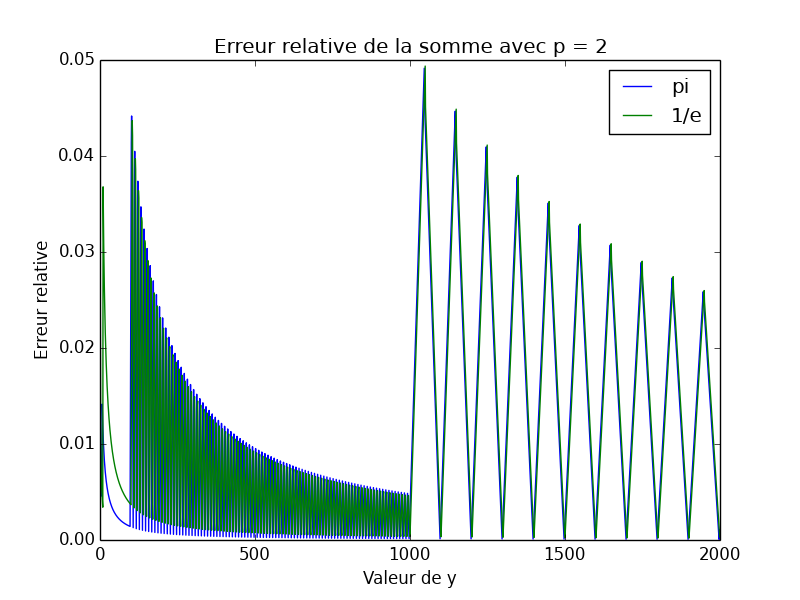
\includegraphics[scale=0.45]{Somme.png}}
  \subfloat[Erreur relative sur le produit]{\label{fig:contour-b}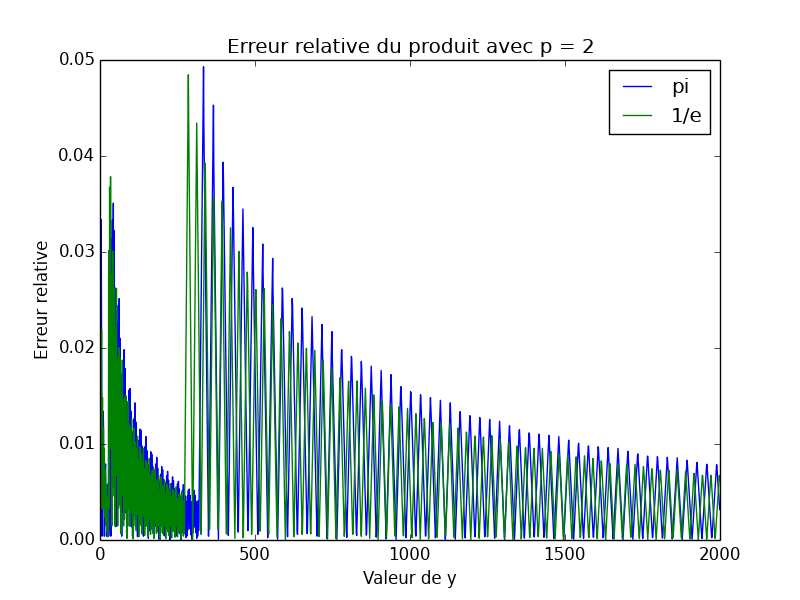
\includegraphics[scale=0.45]{Produit.png}}
  \caption{Erreurs relatives}
  \label{fig:1}
\end{figure}

Les fonctions que nous avons programmé sont d'une part les fonctions \verb1add1 et \verb1prod1 qui s'occupent à partir de nombres et de la précision souhaitée de calculer la représentation réduite respectivement de la somme et du produit. Enfin, les fonctions prenant les même arguments \verb1deltaS1 et \verb1deltaP1 calculent respectivement l'incertitude relative sur la somme et le produit des deux nombre avec la précision donnée.

% subsection hypoth_ses_et_mod_lisation_des_nombres_en_machine (end)
\subsection{Un exemple concret}
Notre objectif consiste maintenant à approcher la valeur de $\log(2)$. Pour cela nous utilisons le développement en série entière de la fonction logarithme décimal, évaluée en $2$ :

\[\log(2)=\sum_{n=1}^{\infty}\frac{(-1)^{n+1}}{n}\]

Une approximation à $p$ décimales consiste à sommer les termes de la somme jusqu'à ce que la différence entre la somme et la valeur réelle soit inférieure à $10^{p-1}$. Soulevons cependant quelques remarques. La première concerne le fait que l'on calcule $\log(2)$ à partir de sa valeur exacte (puisque l'on s'en servirai pour vérifier que l'approximation voulue est atteinte). En pratique, nous n'aurions pas cette possibilité. En conservant cet algorithme, nous pourrions juste nous arrêter dès que la $p$ième décimale est fixée, ceci en vérifiant que la $(p+1)$ième est elle-même fixée. Bien sûr, il s'agit là d'une véritable approximation, puisqu'on ne peut pas savoir avec certitude si en sommant plus loin, la $p$ième décimale ne pourrait pas bouger.\medskip

La bonne solution consiste à exploiter une propriété mathématique des séries alternées, qui consiste à dire que l'erreur sur la somme partielle est inférieure au premier terme du reste (négligé). De façon plus précise, on a que \[|\sum_{i=n+1}^{+\infty}u_i|\le |u_{n+1}|\]. Par conséquent, si l'on veut une précision à la $p$ième décimale, il faudra pousser notre calcul jusqu'au $10^p$ ième terme.\medskip

Autant dire que cette méthode est impraticable même pour des valeurs très faible de $p$. Ainsi, obtenir seulement la $6$ième décimale demande un temps de calcul supérieur à $10$ secondes. D'autre part, les erreurs deviennent rapidemment assez importantes, puisque l'on somme de petites quantités à de grosses quantités, et on perd très rapidemment beaucoup d'informations. Un idée qui a été présentée en cours et que nous avons implémentée, consisterait de sommer à l'envers, en partant des petites quantités, et ce pour conserver leur contribution dans le résultat final. Cependant, le procédé reste toujours aussi improductif...\medskip

Frustrés, nous avons également implémenté l'algorithme d'Aitken-$\delta^2$, qui permet d'obtenir un bonne convergence de cette série, mais il y a une perte de précision avec un grand nombre de sommes partielles initiales. Nous présentons ce procédé dans la deuxième partie.

\begin{function}[H]
    \SetAlgoLined
    \caption{lnDeux(p)}
    \lnDeux{p : entier positif} $\longrightarrow$ $\ln(2)$ à $p$ décimales près, et l'erreur relative cumulée sur la somme\\
    \Deb{
        $y \leftarrow 0$\;
        $i\leftarrow 10^p$\;
        $x\leftarrow 0$\;
        $e\leftarrow 0$\;
        \Tq{$i > 0$}{
            $x \leftarrow (-1)^i \text{prod}(1, \frac{1}{i}, p)$\;
            $e\leftarrow e + \text{deltaS}(x, y, p)$\;
            $y\leftarrow \text{add}(y, x, p)$\;
            $i\leftarrow i - 1$\;
        }
        \Retour{($\text{rp}(y, p)$, $e$)}
    }
\end{function}

\begin{figure}[htp]
  \centering
  \subfloat[Avec une sommation efficace]{\label{fig:edge-c}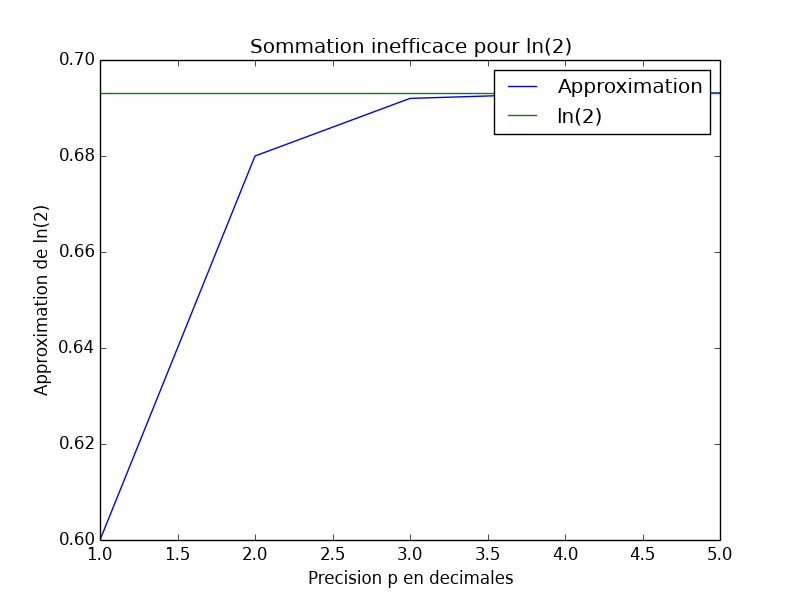
\includegraphics[scale=0.3]{sommation.png}}
  \subfloat[Erreur relative]{\label{fig:contour-d}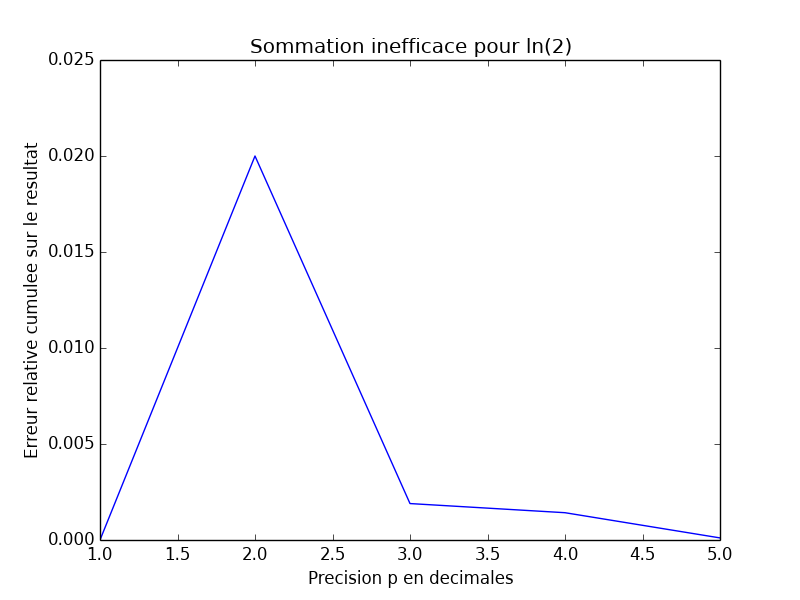
\includegraphics[scale=0.3]{sommation_erreur.png}}
  \subfloat[Avec Aitken]{\label{fig:contour-e}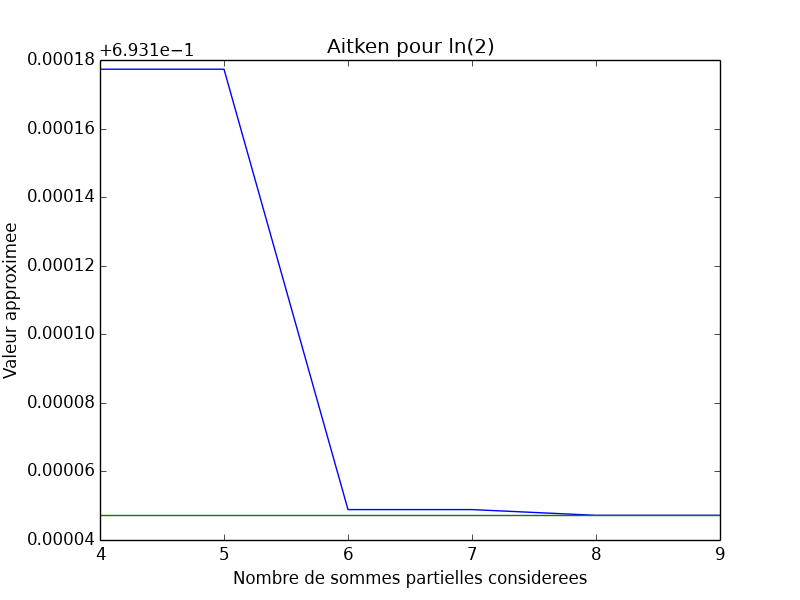
\includegraphics[scale=0.3]{Aitken.png}}
  \caption{Précision des algorithmes de calculs de $\ln(2)$}
  \label{fig:2}
\end{figure}

Que peut-on conclure de ces implémentations. La première conclusion est que la rapidité de convergence est essentielle pour obtenir des résultats corrects et éviter de multiplier les opérations et donc de multiplier les erreurs ! Ce qui fait partie de la complexité en temps de l'algorithme. D'autre part, on vérifie effectivement la majoration des erreurs, qui traduit le fait que plus $p$ est grand, plus le résultat est précis.

% section repr_sentation_des_nombres_en_machine (end)
\section{Algorithme CODRIC}
\subsection{Représentation sur une calculatrice}
Les calculatrices ne sont pas aussi puissantes que les ordinateurs, nous cherchons maintenant à savoir ce qui se produit au niveau de ces machines pour l'évaluation de quelques fonctions élémentaires.

Dans la plupart des calculatrices, un nombre flottant sur huit octets est représenté par :
\begin{itemize}
    \item m : une mantisse constituée de treize chiffres codés indépendamment sur quatre bits soit 52 bits au total;
    \item e : un exposant (en puissance de 10) éventuellement signé sur 11 bits;
    \item s : le signe du nombre (et de l'exposant s'il n'est pas signé) sur 1 bits.
\end{itemize}

Cette représentation est certes efficace car elle permet de représenter avec une bonne précision les flottants, cependant, celle-ci est invalide pour des valeurs trop grandes, il y a risque d'\textit{overflow}. Notons également que les approximations cumulées aboutissent en fin de compte à une imprécision assez importante.


\subsection{Fonctions trigonométriques}
 Lors de l'implémentation des fonctions trigonométriques, il se pose un problème quant à l'efficacité des approximations effectuées. Nous avons implémenté les fonctions $\ln$, $\exp$, $\tan$ et $\text{Arctan}$. La méthode choisie consiste à approximer ces fonctions pour des valeurs comprises dans de très petits intervalles, à partir de valeurs remarquables connues. Ainsi pour calculer l'évaluation de la fonction à une valeur donnée, il suffit de la ramener judicieusement dans un intervalle précis pour lequel on pourra exprimer la valeur de l'évaluation en fonction des évaluations rpé-enregistrées de la fonction.

Cette méthode est très efficace pour les calculatrices. En effet, vu la simplicité et le faible nombre des opérations effectuées, l'erreur commise est limitée, le tout avec une occupation en espace due aux valeurs pré-enregistrée très faible.

Pour tester ces fontions, nous avons utilisé certaines propriétés qui leur étaient propres, pour la fonction $ln$ par exemple, il s'agissait de calculer la valeur de $ln(1)$ et de s'assurer que l'on a bien la valeur $0$.

Nous avons également vérifié les propriétés suivantes :

\begin{itemize}
\item $ \exp ( a + b) = \exp(a)*\exp(b)$

 
\item$ \ln ( a*b)= \ln(a) + \ln(b)$

 
\item$\text{Arctan}(x)+ \text{Arctan}(1/x) = \pi/2 $


\item$\tan(x + \pi/2 ) = -1/\tan (x) $
\end{itemize}
Ces propriétés sont vérifiées avec nos fonctions. Nous aurions pu pousser nos tests plus loin, mais nous nous sommes contentés de vérifier la parfaite superposition des graphes générés et avec ceux des fonctions associées.

\subsection{Evaluation de fonctions}
Lorsqu'on souhaite évaluer des fonctions, on a toujours un certain degré d'imprécision à gérer.

Un problème qui met en évidence ces erreurs est l'évaluation de la convergence des séries.

Le développement en série de Taylor d’une fonction est un bon moyen d’approximer la dite fonction par une série entière au voisinage d’un point $x_0$ .

\[f(x)=\sum_{k=0}^\infty~\ a_k(x-x_0)^k\]

Cependant, une série étant une somme infinie, il faut arrêter de sommer les termes au bout d’un certain temps, et c’est la que réside le problème : Au bout de combien de termes  sommes-nous sûrs d'avoir la précision attendue ? Il serait donc pratique d’essayer d’accélérer la vitesse de convergence de la série.

Pour cela nous disposons de plusieurs moyens. Si la série considérée a une convergence approximativement géométrique, on peut extrapoler les sommes partielles de proche en proche.

On a :
\begin{equation}
S'_n = S_{n+1} - \frac{(S_{n+1} - S_n)^2}{S_{n+1} -2S_n + S_{n-1}}
\end{equation}

Cependant certaines séries ne peuvent pas être accélérées par cette méthode, comme le développement en série entière du sinus, car elle converge partout mais jamais assez vite pour être exploitée de manière numérique.

\[\sin(x)=\sum_{n=0}^\infty~\frac{(-1)^k}{(2k+1)!} x^{2k+1}\]

D'autre part, si la série considérée est alternée, on peut utiliser la transformation d'Euler.

Un autre problème consiste en l'évaluation du module des nombres complexes.

L'évaluation du module d’un nombre complexe est relativement aisée de manière mathématique avec l’expression \[|a + ib| = \sqrt{(a^2 + b^2})\], mais il en va autrement de manière numérique.

En effet, parce-que l'on met des nombres au carré, il peut subvenir rapidement un \textit{overflow} des que $a$ ou $b$ va dépasser une certaine valeur pas forcémment très importante, alors que l'on peut facilement gérer des nombres complexes avec des valeurs de $a$ ou $b$ bien plus élevées par le calcul de l'expression suivante, qui nécessite des calculs intermédiaires ne dépassant pas l'ordre de grandeur de $a$ ou de $b$, et par conséquent, évite tout \textit{overflow} :

\[|a + ib| = \left\lbrace\begin{array}l |a|  \sqrt{(1 + (b/a)^2} \rm~~si~ | a | \ge |b|  \\ | b |  \sqrt{(1 + (a/b)^2}\rm~~si~ | a | \leq | b |\end{array}\right. \]

Enfin l’évaluation de la dérivée d'une fonction grâce au taux d’accroissement \[ f'(x) \approx \frac{f(x+h)-f(x)}{h}\] peut donner un résultat inexact suite à la troncature et à l’arrondi. Ils interviennent dans le développement de Taylor de $f$ ainsi que dans le choix des valeurs pour $x$ et $h$. 

Une amélioration de précision peut être obtenue avec l’expression \[ f'(x) \approx \frac{f(x+h)-f(x-h)}{2h}\] (qui nécessite néanmoins des performances de calculs plus élevées car on évalue deux fois la fonction.)\bigskip


\ \\
\textbf{\textsc{Conclusion :}}

Ce projet nous a permis, outre le fait de nous familiariser avec le langage \textit{Python}, de prendre conscience de la difficulté de représenter des nombres en machine, de la facilité de tomber dans tous leurs travers dès qu'on les manipule et enfin de voir les moyens utilisés pour garantir des approximations plus efficaces lors de différents calculs numériques.
\end{document}
